\subsection{Translational Force Measurement via Angular Deflection}

\subsubsection{Laboratory Simulation with Solenoid Coil}

To assess MRI-induced translational forces in a laboratory environment, Creighton University developed a pendulum-style apparatus following the geometry and physics outlined in ASTM F2052-15\cite{astmF2052}. The vertical post includes a screw clamp mechanism that enables height adjustment; however, a default suspension height of 1 meter was used for consistency across trials.

The experimental frame was constructed entirely from \gls{pvc} components (Figure \ref{fig:schematic}a), including a vertical post of 1.5 meters and a rigid base for stabilization. The sample—a \textbf{solid ferromagnetic cylinder} (length = 6 mm, diameter = 3 mm, mass = 0.3648 g, density = 8.6 g/cm$^3$)—was suspended by a \textbf{955 mm-long sewing thread}, tied via a simple knot at its center. For clinical applications, a \textbf{0.25 mm nylon monofilament} is recommended for improved reproducibility and safety. A Monofilament Nylon thread has low stretch,  complies with MR-safe properties (Non-metallic, Non-conductive, Non-magnetic), and reduces variability introduced by torsional drift or thread elasticity  \cite{stoianovici2024, astmF2052}. The bottom of the sample was free to swing, forming a pendulum under gravity. A horizontal ruler, fixed along the Z-axis, served as the visual reference to quantify lateral displacements as shown in Figure \ref{fig:schematic}b and detailed in Figure~\ref{fig:leadcloseup}. 


\begin{figure}[H]
	\centering
	\begin{minipage}[b]{0.48\textwidth}
		\centering
		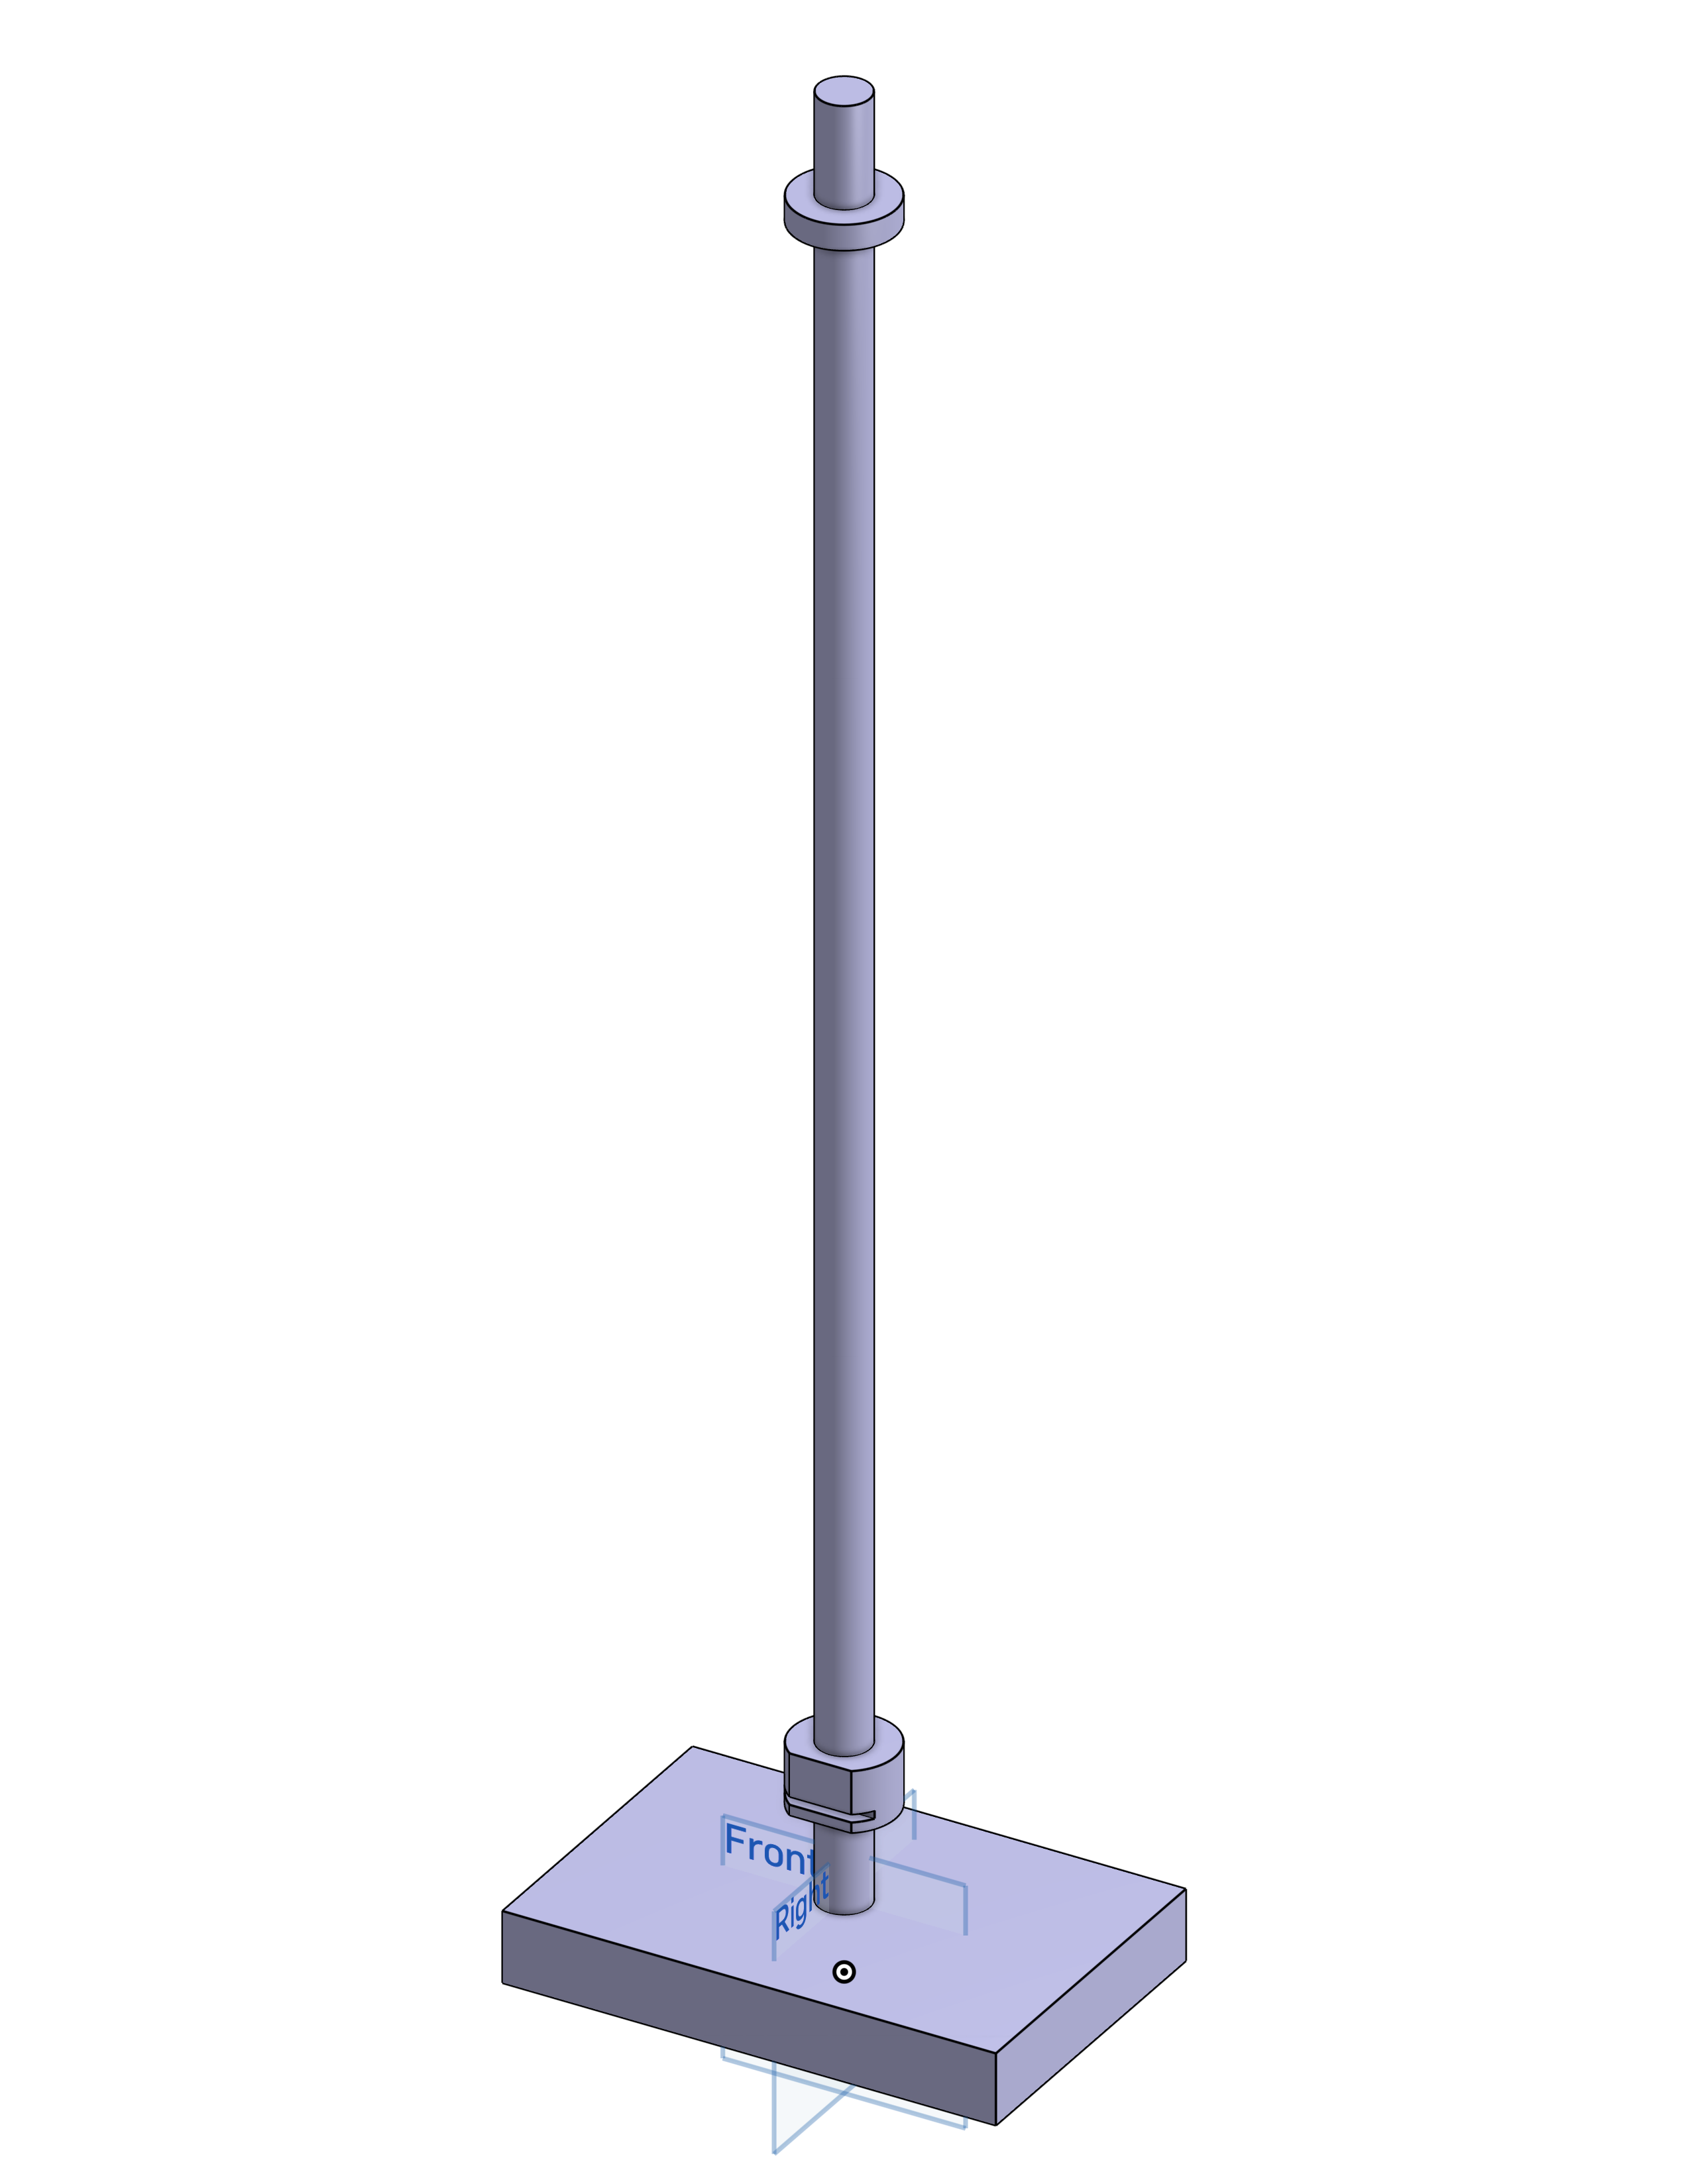
\includegraphics[width=\textwidth]{Assests/Part1.png}
		\subcaption{CAD render of the pendulum apparatus created using CATIA.}
	\end{minipage}
	\hfill
	\begin{minipage}[b]{0.48\textwidth}
		\centering
		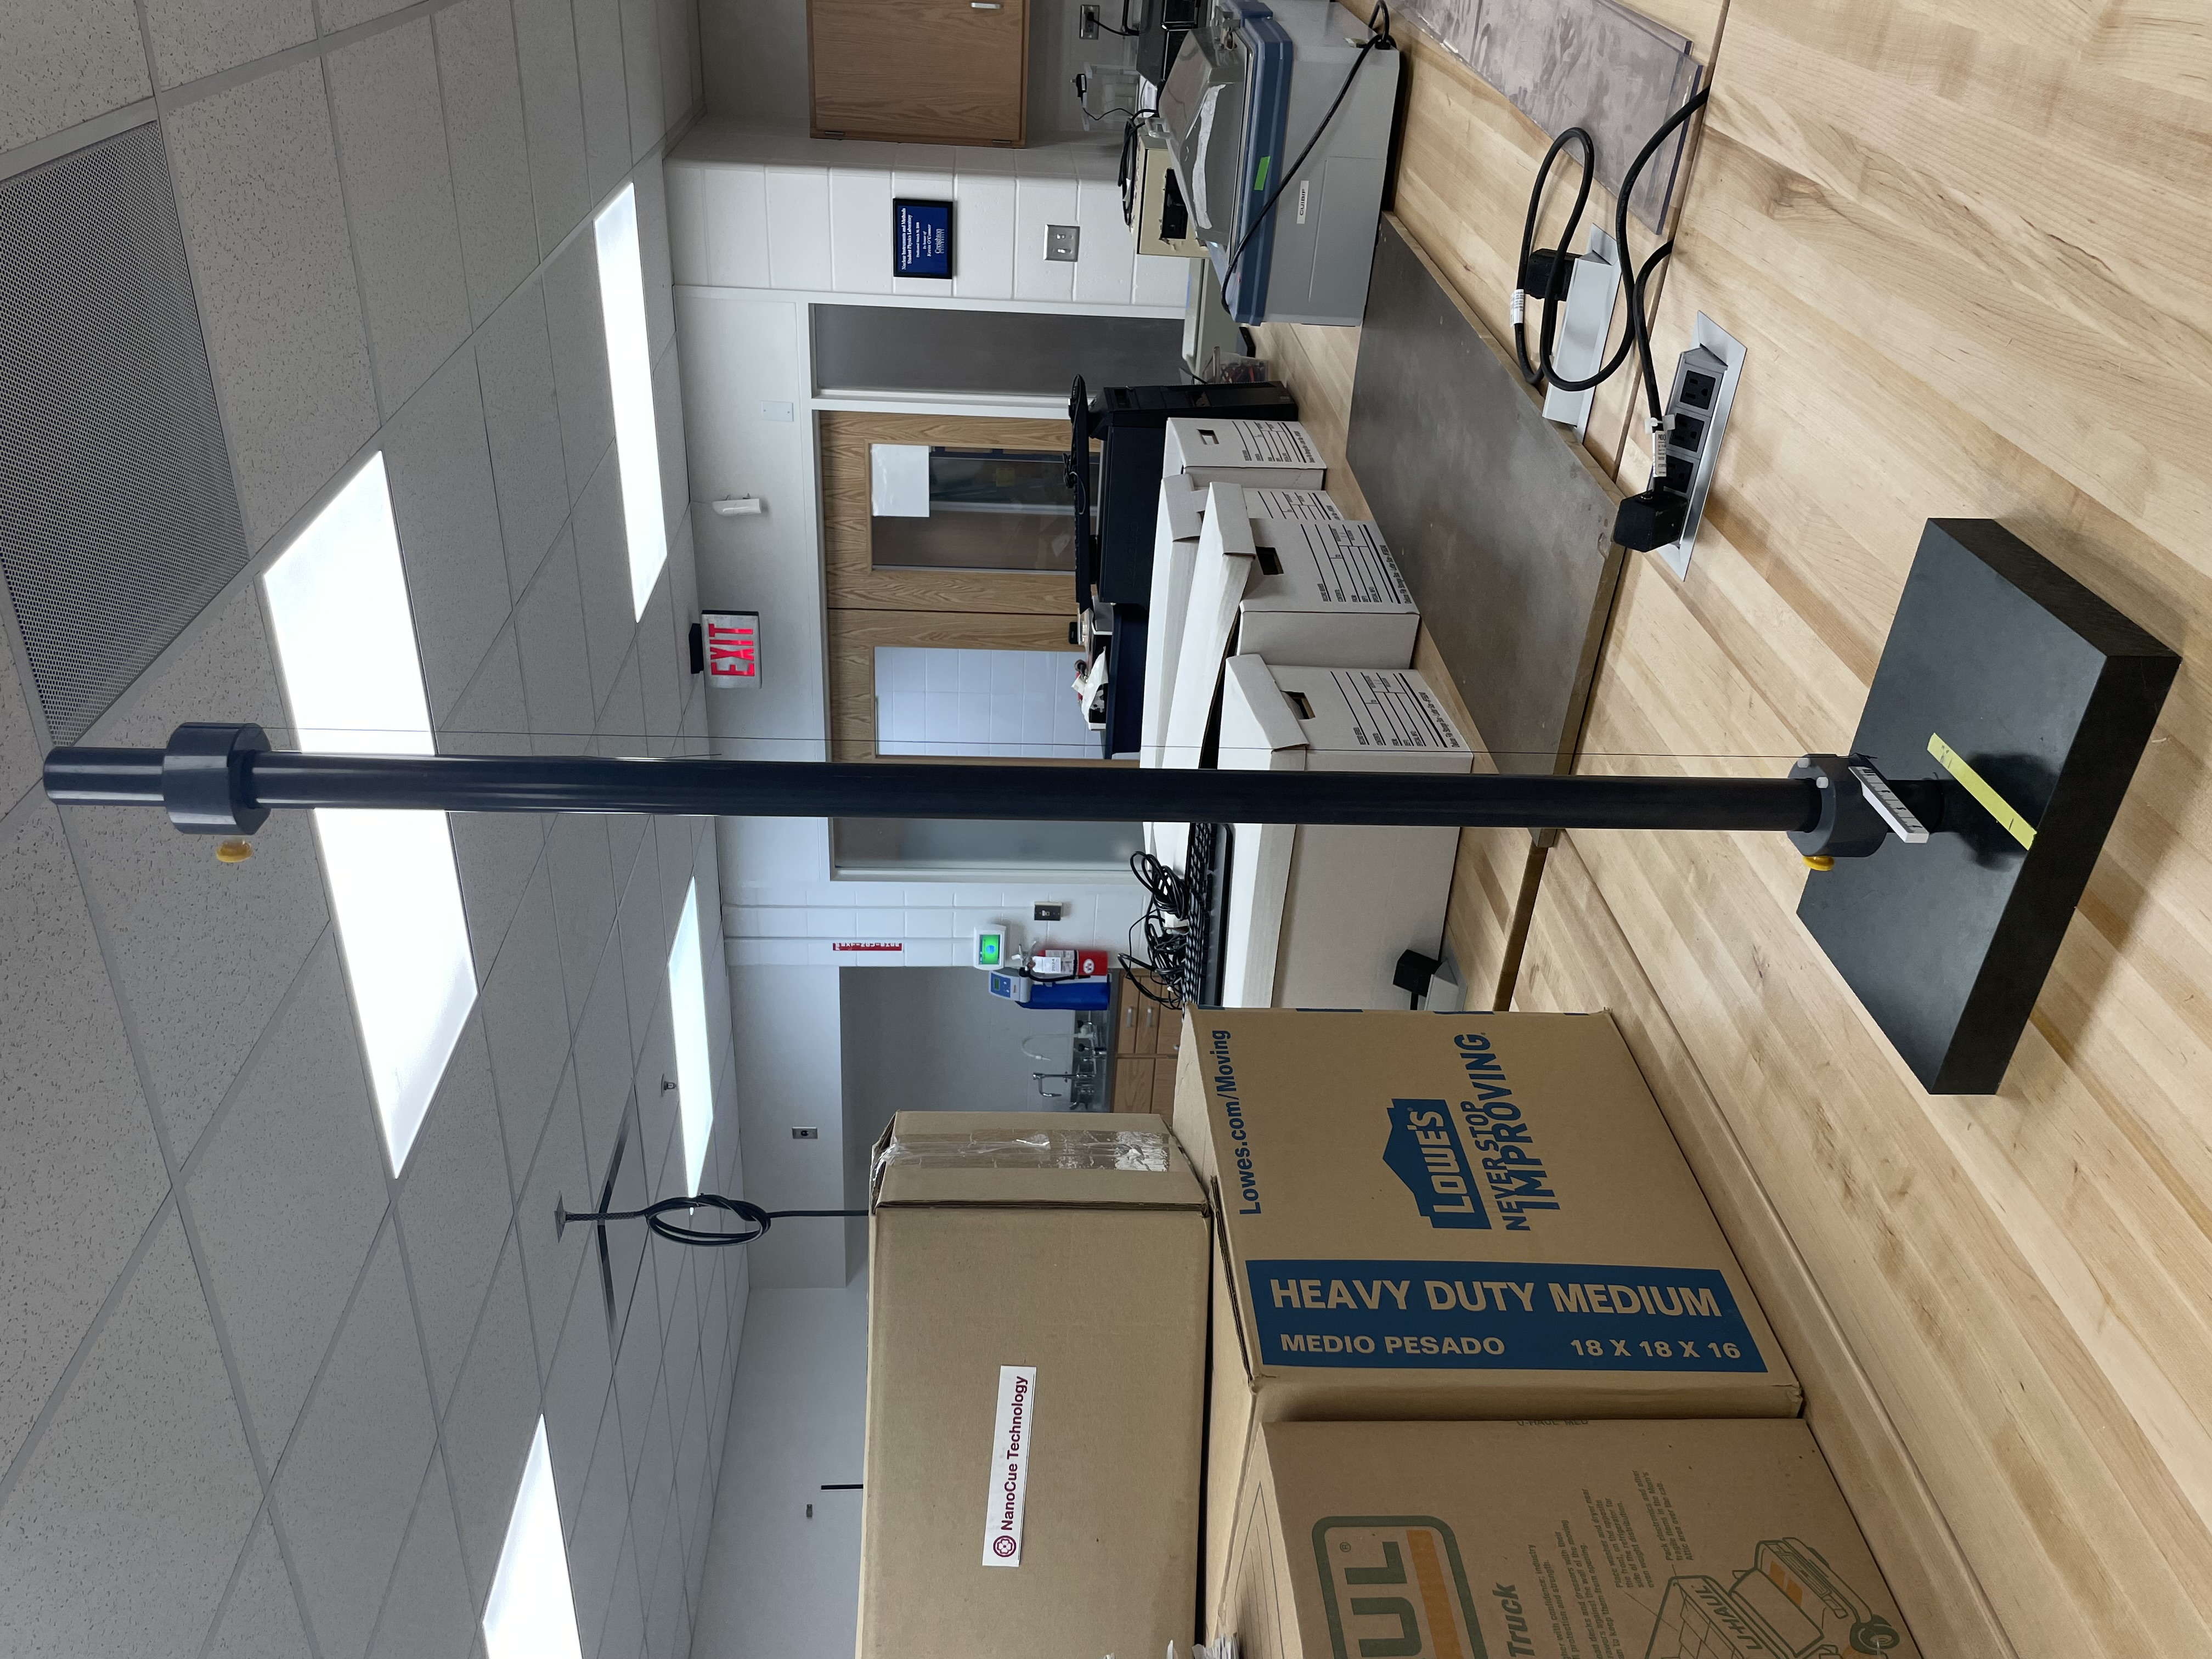
\includegraphics[width=1.3\textwidth, angle=-90]{Assests/Picture1.jpg}
		\subcaption{Real-life implementation of the apparatus in the laboratory setting.}
	\end{minipage}
	\caption{Experimental pendulum-based apparatus constructed from PVC for MRI translational force measurements.}
	\label{fig:schematic}
\end{figure}

\subsubsection*{Lead Holder Frame Design}

To accommodate epicardial lead positioning while maintaining MRI compatibility, we propose the use of a lightweight, non-magnetic bee comb mesh also fabricated from \gls{pla}. The suggested mesh dimensions are 16 mm length by 14 mm wide, with a thickness of 1 mm, for a total volume of less than $100 mm^3$ equivalent to around a tenth of 1 gram given the 1.24 grams per cubic centimeter ($g/cm^3$) \gls{pla} density. 

As shown in figure \ref{fig:leadHolder} and \ref{fig:leadcloseup}.

The mesh needs to be suspended such that the lead axis was aligned approximately parallel to the magnetic field gradient (Z-axis). The mesh's lightweight design aimed to minimize its contribution to the total magnetic force, however its mass was not explicitly subtracted from the translational force calculations.

\begin{figure}[H]
	\centering
	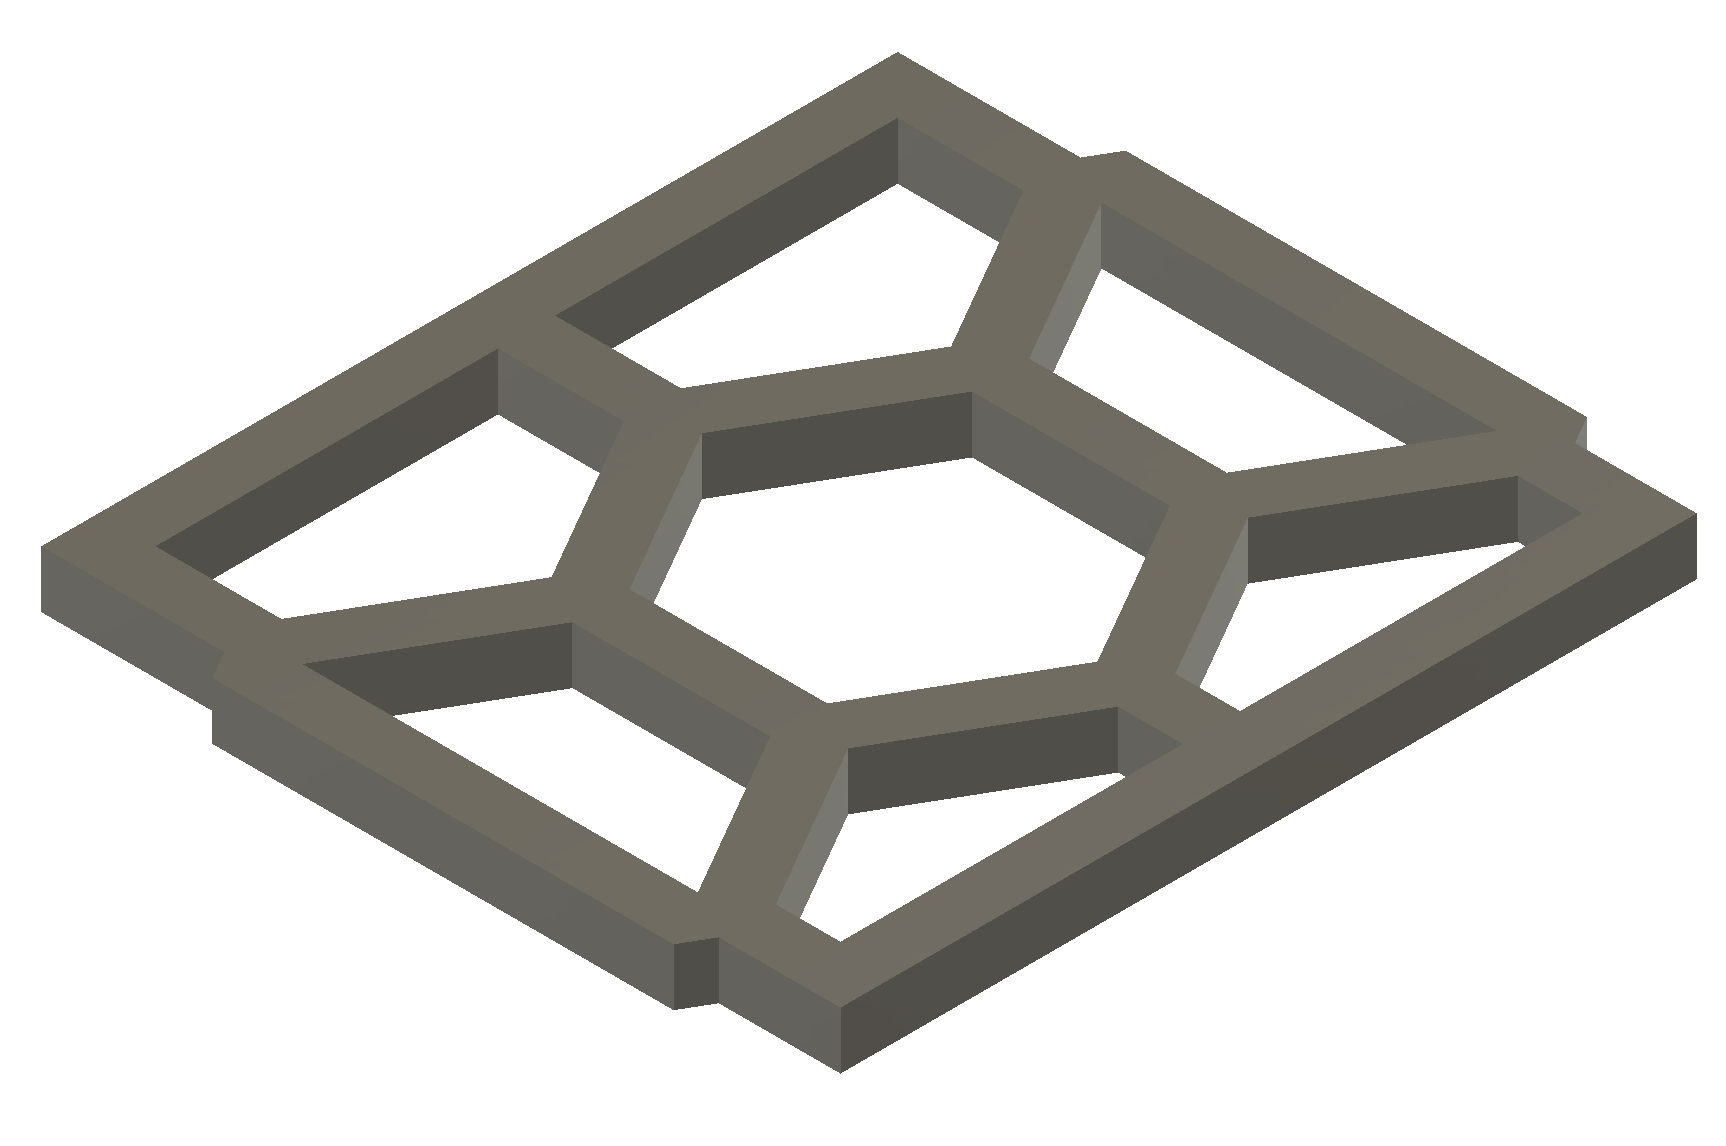
\includegraphics[width=0.5\textwidth]{Assests/frameHolder.png}
	\caption[3D render of the design on lead holder]{The design on lead holder comprises a rectangular lightweight bee comb mesh to wrap the epicardial lead around and hold it in a pendulum with a nylon string}	
	\label{fig:leadHolder}
\end{figure}

A summary schematic of the apparatus and frame are included in Figures \ref{fig:schematic} and \ref{fig:leadHolder}, with additional engineering drawings available in %\textbf{\AppendixAone} and \textbf{\AppendixAtwo}.



\begin{figure}[H]
	\centering
	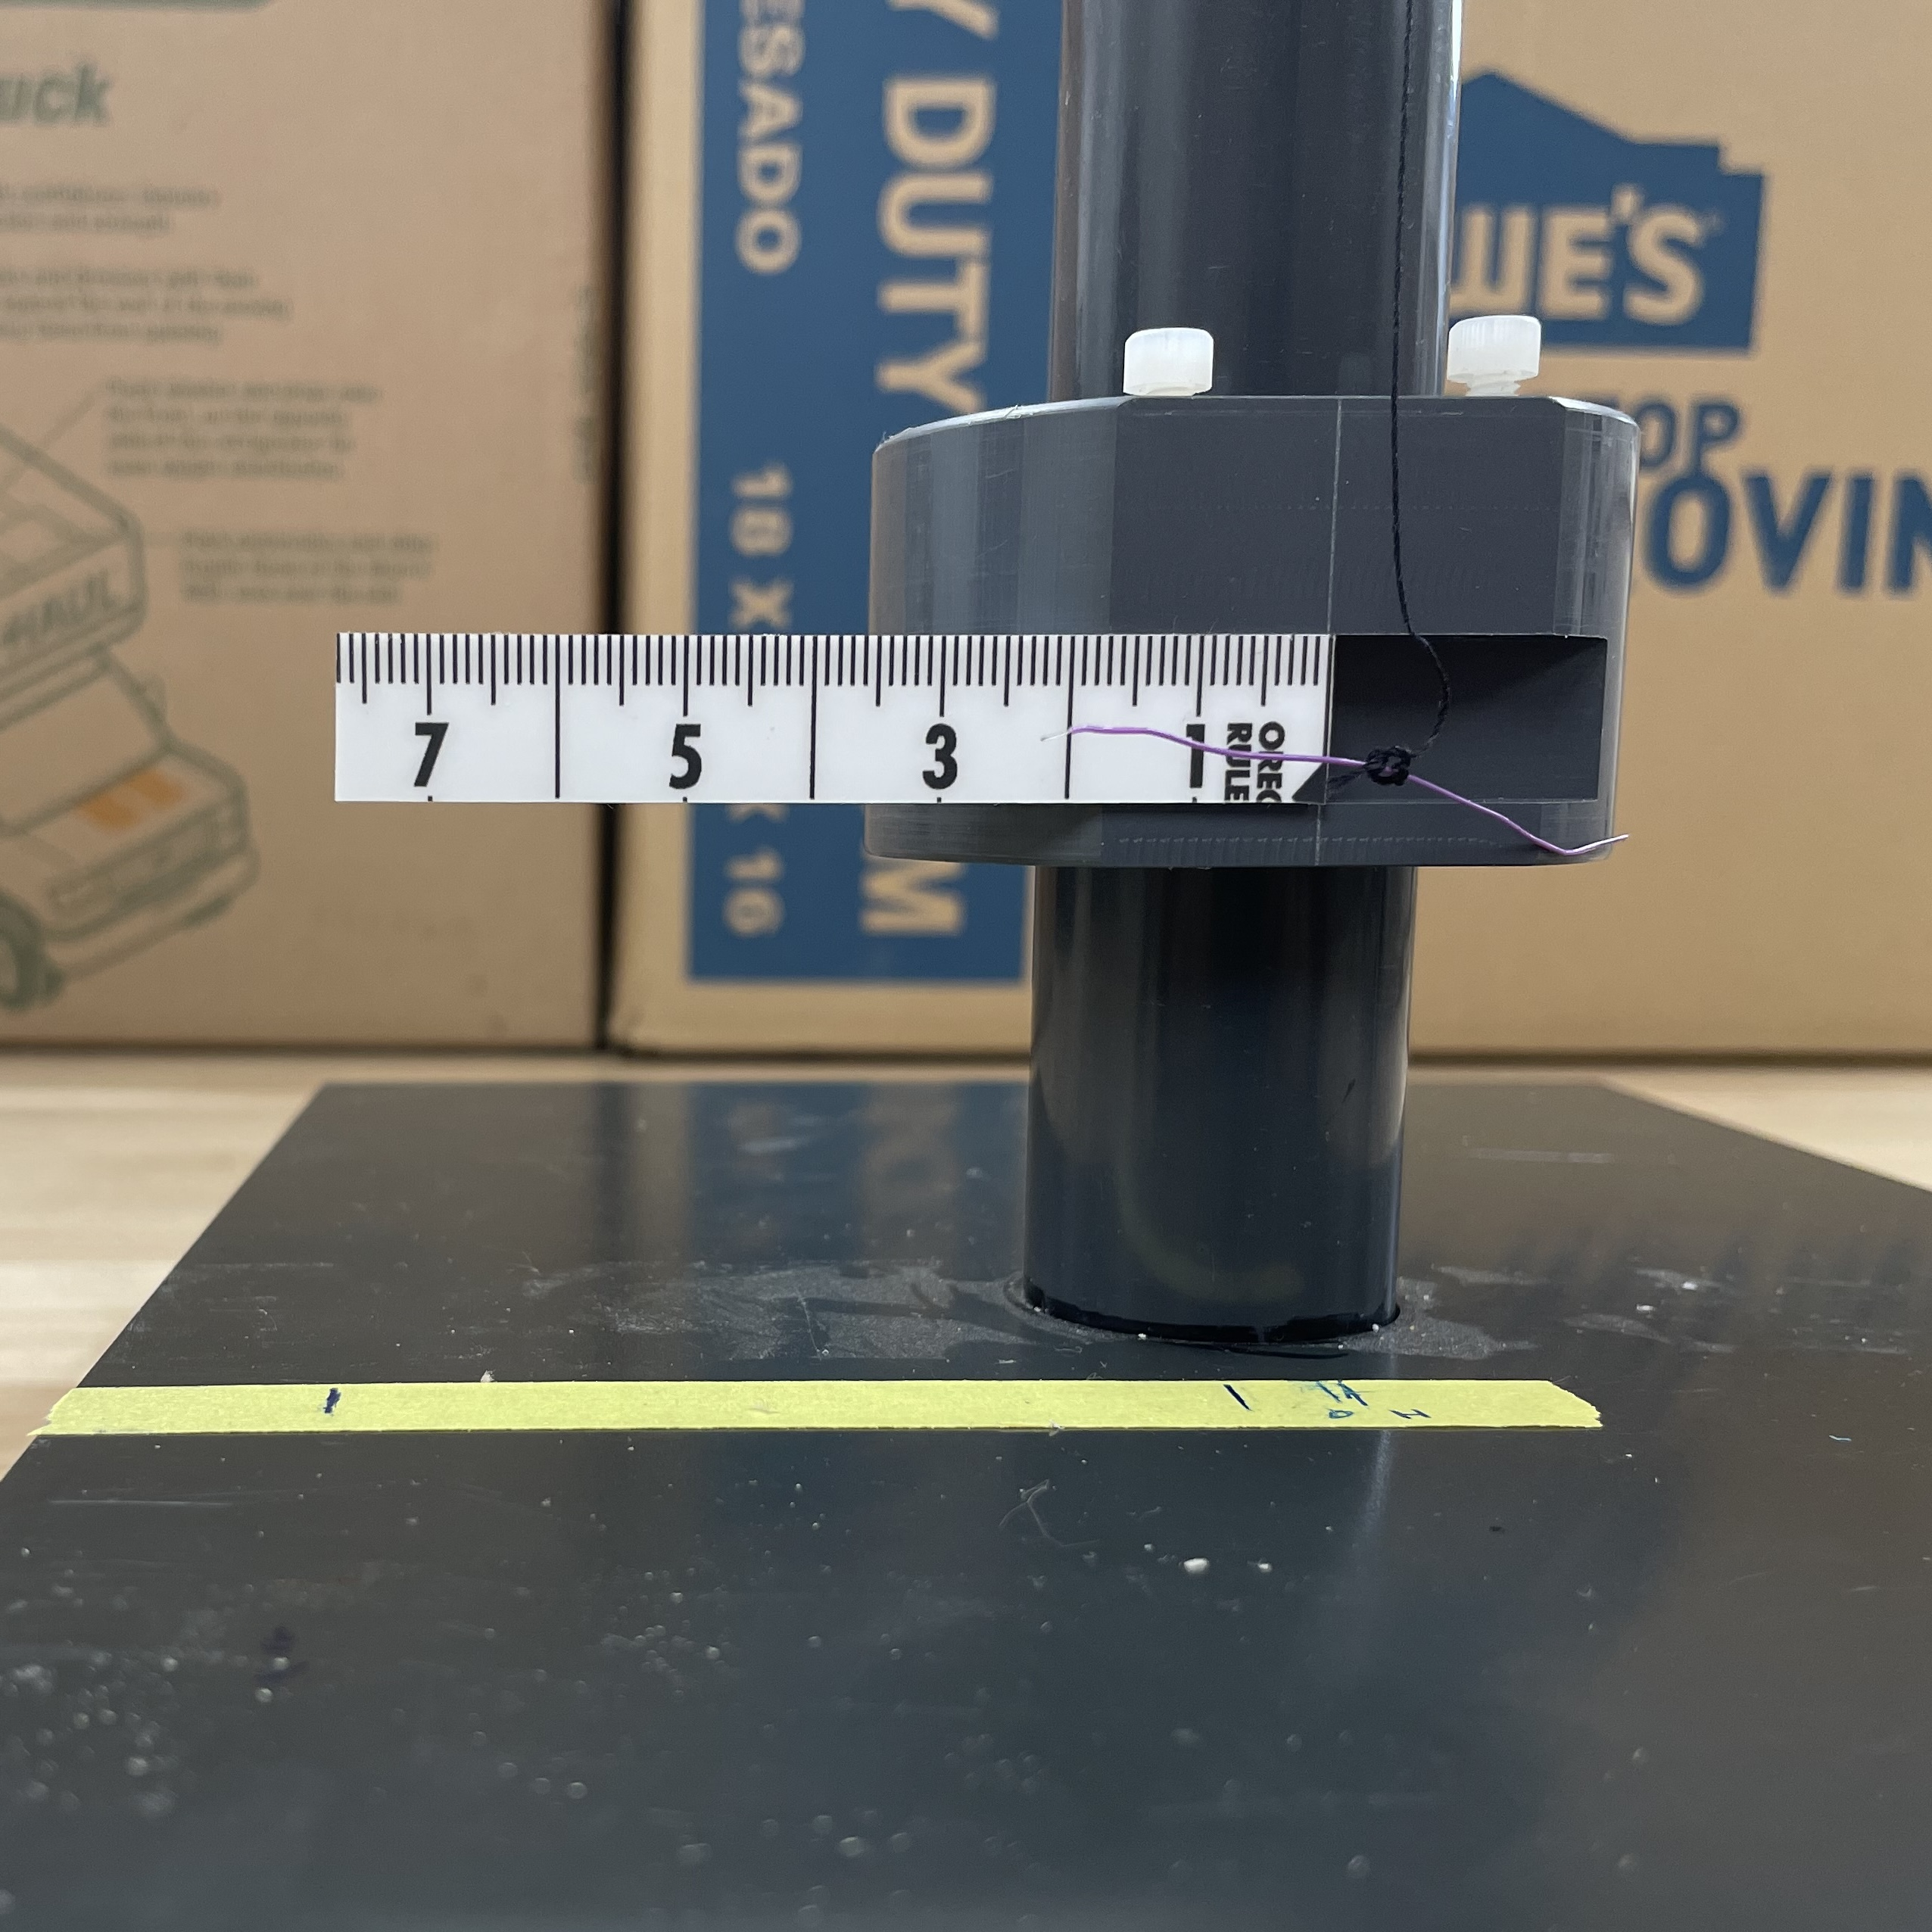
\includegraphics[width=0.6\textwidth]{Assests/Picture2.jpg}
	\caption{Close-up of the epicardial lead fragment suspended by monofilament thread over the ruler. Image illustrates the displacement measurement system and the sample scale.}
	\label{fig:leadcloseup}
\end{figure}

\subsubsection*{In Lab Measurement Protocol}

Magnetic field measurements were performed using the \textbf{AlphaLab Inc. Gaussmeter} described before. To characterize local field gradients, measurements were taken at three positions: at the pendulum's equilibrium position, 0.5 mm below, and 0.5 mm above, yielding values of $B_{-0.5}$, $B_0$, and $B_{+0.5}$, respectively. Each position was sampled \textbf{nine times per current level}, and gradients were computed using python pandas library and the central finite difference method:

\begin{equation}
	\frac{dB}{dz} \approx \frac{B_{+0.5} - B_{-0.5}}{1\ \text{mm}}
\end{equation}

Once the pendulum reached equilibrium under each magnetic condition, the horizontal displacement on $z$ was recorded visually using the ruler as a reference. With known suspension length $L$, the \textbf{deflection angle $\alpha$} was calculated as:

\begin{equation}
	\alpha = \tan^{-1}\left(\frac{x}{L}\right)
\end{equation}

Following ASTM F2052-15, the translational force exerted on a device due to a static magnetic field spatial gradient can be evaluated through angular deflection. In this setup, the test object is suspended in equilibrium, and the balance of forces leads to:

\begin{equation}
	\tan \alpha = \frac{F_m}{mg}
\end{equation}

where $\alpha$ is the deflection angle from vertical, $F_m$ is the magnetically induced translational force, $m$ is the mass of the object, and $g$ is the gravitational acceleration. Rearranging gives:

\begin{equation}
	F_m = mg \tan \alpha
\end{equation}

This is also derived from Newtonian force balancing as in Appendix X2 of ASTM F2052-15 (Fig \ref{fig:astm_diagram}), and is valid even in cases when the magnetic force does not operate exactly at the center of mass. As a result, the approach is reliable for evaluating a variety of devices.

\begin{figure}[htbp]
	\centering
	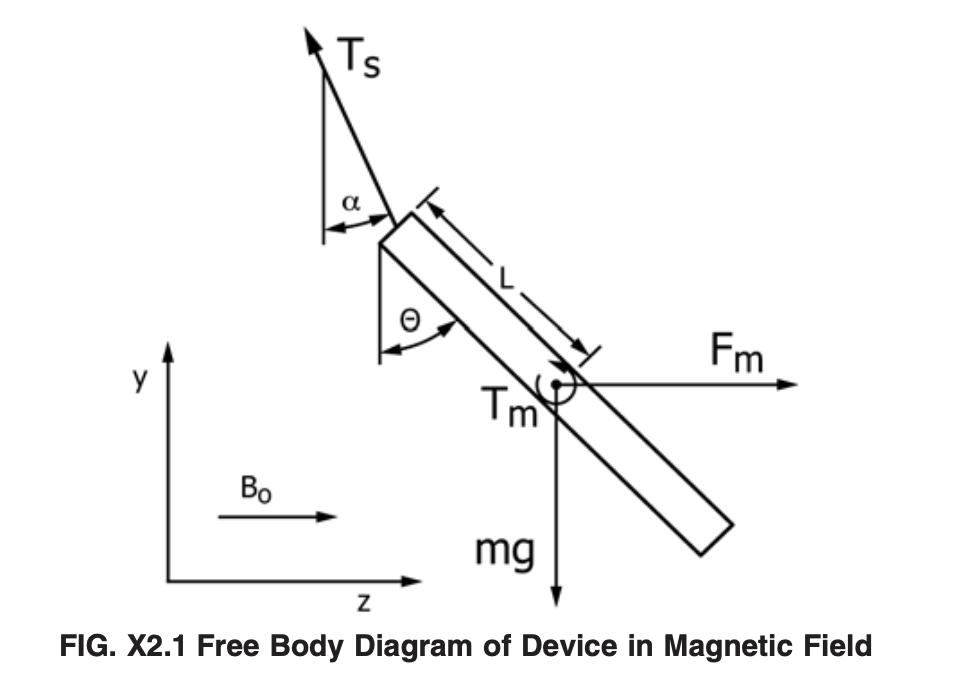
\includegraphics[width=0.6\textwidth]{Assests/astm_diagram.png}
	\caption{Free-body diagram of device in magnetic field (adapted from ASTM F2052-15, Appendix X2).}
	\label{fig:astm_diagram}
\end{figure}

For materials where magnetization is induced by a static field (e.g., paramagnetic or unsaturated ferromagnetic materials), the translational force can also be expressed in terms of volumetric magnetic susceptibility $\chi$, assuming linear response:

\begin{equation}
	F_m = \frac{\chi V}{\mu_0} B_0 \frac{dB_0}{dz}
	\quad \Rightarrow \quad
	\chi = \frac{\mu_0 F_m}{V B_0 \frac{dB_0}{dz}}
\end{equation}

Combining this with the earlier result:

\begin{equation}
	\chi = \frac{\mu_0 m g \tan \alpha}{V B_0 \frac{dB_0}{dz}}
\end{equation}

This provides a direct estimation of magnetic susceptibility from angular deflection measurements, provided the field and its gradient are known. 

The ratio is expressed as follows using a different, dimensionally reduced form from ASTM F2052-15's Appendix X3:

\begin{equation}
	\frac{\chi}{\rho \mu_0 g} = \frac{\tan \alpha}{B_0 \frac{dB_0}{dz}}
\end{equation}

This formulation explains why the measured deflection angle $\alpha$ (and thus $F_m$) depends not on $\chi$ or $B_0$ independently, but on their product. Practically, this insight justifies our lab methodology: although our solenoid generates only ~20 Gauss, we used a highly ferromagnetic sample (large $\chi$), allowing us to replicate clinically relevant force-to-weight ratios ($F_m / mg$).

In the clinical MRI environment, $B_0$ may reach 3 T, but the $\chi$ of implanted materials is often orders of magnitude smaller. This inverse balance preserves the translational force regime, and supports translating results from lab simulations to clinical conditions.

%\subsection*{Data Collection and Analysis}

All measurements were logged in \textbf{Microsoft Excel}, and photos/videos were captured via smartphone to document behavior. A minimum of \textbf{three trials} were performed for each current level; however, only the final (most consistent) dataset was retained for analysis. Data were exported to a Jupyter Notebook for clean up and processing with pandas. Then plotted to evaluate $\tan \alpha$ vs. field gradient force. Propagated uncertainties in $\alpha$ and $dB_0/dz$ were computed using standard error propagation formulas.

\subsubsection{In Clinic Measurement Protocol}


